
% Template by Arnau, based on:
%%%%%%%%%%%%%%%%%%%%%%%%%%%%%%%%%%%%%%%%%
%
% Beamer Presentation
% LaTeX Template
% Version 1.0 (10/11/12)
% This template has been downloaded from:
% http://www.LaTeXTemplates.com
% License:
% CC BY-NC-SA 3.0 (http://creativecommons.org/licenses/by-nc-sa/3.0/)
%%%%%%%%%%%%%%%%%%%%%%%%%%%%%%%%%%%%%%%%%


%----------------------------------------------------------------------------------------
%	PACKAGES AND THEMES
%----------------------------------------------------------------------------------------

\documentclass[.08pt,aspectratio=169,t]{beamer}
% \usefonttheme{serif}
%% serif
%% professionalfonts
%% structurebold
%% structureitalicserif
%% structuresmallcapsserif

\mode<presentation> {

\usetheme{Boadilla}

% As well as themes, the Beamer class has a number of color themes
% for any slide theme. Uncomment each of these in turn to see how it
% changes the colors of your current slide theme.
\usecolortheme{seahorse}  % The them I usually use, because it resembles the PSI template.

%\setbeamertemplate{footline} % To remove the footer line in all slides uncomment this line
%\setbeamertemplate{footline}[page number] % To replace the footer line in all slides with a simple slide count uncomment this line
}

\setbeamertemplate{sections/subsections in toc}[sections numbered]  % Controls style of number in the table of contents.

% Packages:
\usepackage{adjustbox}
\usepackage{algorithm}
\usepackage{algpseudocode}
\usepackage{amsmath,amsfonts,amsthm,amssymb}
\usepackage{pdfrender}
\usepackage{animate}
\usepackage{appendixnumberbeamer}
\usepackage{booktabs} % Allows the use of \toprule, \midrule and \bottomrule in tables
\usepackage{cancel}
%\usepackage{dutchcal}
\usepackage{enumitem, bbding}
\usepackage{float}
\usepackage{graphicx} % Allows including images
\usepackage{hhline}
\usepackage{listings}
\lstset{
  language=Python,
  basicstyle=\ttfamily,
  mathescape
}
\usepackage{mathtools}
\usepackage{multicol}
\usepackage{multimedia}
\usepackage[authoryear]{natbib}
\usepackage{scrextend}
\changefontsizes{9pt}
\usepackage{siunitx}
\usepackage{soul}
\usepackage{tikz}
\usetikzlibrary{mindmap, trees, arrows, shapes, backgrounds, matrix, decorations.pathreplacing, decorations.pathmorphing, positioning, arrows.meta,plotmarks, calc}
\usepackage{verbatim}
\usepackage{xmpmulti}
\usepackage{ulem}

% Bold Math
\usepackage{bm}
\usepackage[font=footnotesize]{caption}
% Dashed horizontal lines
\usepackage{arydshln}
% For spacing between underbrace and text
% \addstackgap[6pt]
\usepackage{IEEEtrantools,stackengine}

% \bibliographystyle{unsrt}  % This style cites with numbers, e.g. [2]
\bibliographystyle{unsrtnat}  % This style cites with names, e.g. [Adelmann, 2019]

% Code Listing
\usepackage{listings}
\usepackage{color}

\definecolor{dkgreen}{rgb}{0,0.6,0}
\definecolor{gray}{rgb}{0.5,0.5,0.5}
\definecolor{mauve}{rgb}{0.58,0,0.82}

\lstset{frame=tb,
  language=C++,
  aboveskip=3mm,
  belowskip=3mm,
  showstringspaces=false,
  columns=flexible,
  basicstyle={\small\ttfamily},
  numbers=none,
  numberstyle=\tiny\color{gray},
  keywordstyle=\color{blue},
  commentstyle=\color{dkgreen},
  stringstyle=\color{mauve},
  breaklines=true,
  breakatwhitespace=true,
  tabsize=3
}


%%%%%%%%%%%%%%%%%%%%%%%%%%%%%%%%%
% Tikz stuff:
\usetikzlibrary{positioning}
\usetikzlibrary{patterns}
\usetikzlibrary{shapes}
\usetikzlibrary{matrix, arrows,decorations.pathmorphing}
\usetikzlibrary{decorations.markings}
\usetikzlibrary{fadings}
\usetikzlibrary{arrows.meta,bending}
\usepackage{tikzscale}
%%%%%%%%%%%%%%%%%%%%%%%%%%%%%%%%%
%%%%%%%%%%%%%%%%%%%%%%%%%%%%%%%%%


\setbeamertemplate{navigation symbols}{}  % Remove navigation symbols
\setbeamersize{text margin left=1cm,text margin right=1cm}

%% Maths definitions.
\DeclareMathOperator*{\argmin}{arg\,min}
\DeclareMathOperator*{\supp}{supp}
\DeclareMathOperator*{\Var}{\mathrm{Var}}
\DeclareMathOperator*{\Cov}{\mathrm{Cov}}
\DeclareMathOperator*{\E}{\mathbb{E}}
\DeclareMathOperator*{\MSE}{\text{MSE}}
\DeclareMathOperator*{\sgn}{\text{sgn}}
\DeclareMathOperator*{\Epsilon}{\mathcal{E}}
\DeclareMathOperator*{\bigO}{\mathcal{O}}
\DeclareMathOperator*{\smalls}{s}
\newcommand{\mvec}[1]{\boldsymbol{#1}}
\newcommand\underrel[2]{\mathrel{\mathop{#2}\limits_{#1}}}

%% Rendered Symbols
\newcommand*{\boldcheckmark}{%
  \textpdfrender{
    TextRenderingMode=FillStroke,
    LineWidth=.5pt, % half of the line width is outside the normal glyph
  }{\checkmark}%
}

%----------------------------------------------------------------------------------------
%	TITLE PAGE
%----------------------------------------------------------------------------------------

%%%%%%%%%%%%%%%%%%%%%%%%%%%%%%%%%%%%%%%%%
% Enter here author information:
\title[]{The Langevin Approach to Discretize the Collision Operator} % The short title appears at the bottom of every slide, the full title is only on the title page.

\author{\textbf{Tobia Claglüna}}
\institute[LSM, PSI]{Midterm Presentation\\}
%\date{\today}
\def \myEmail {tobiac@ethz.ch}
%%%%%%%%%%%%%%%%%%%%%%%%%%%%%%%%%%%%%%%
\newcommand{\frametitlepsi}[1]{\frametitle{\hspace{0.8cm}
\includegraphics[width=1.5cm]{logos/PSI.pdf}\hspace{1.1cm} #1}}

\begin{document}
\setbeamertemplate{caption}{\raggedright\insertcaption\par}
\def\vfilll{\vskip 0pt plus 1filll minus 0pt }
\begin{frame}
  % Title page image:
  \vspace{0.3cm}
  \begin{adjustbox}{width=\paperwidth, center}
    \begin{tikzpicture}
      \centering
      \filldraw[fill=lightgray!40!white, draw = none] (0,0) rectangle (3.3,0.5\textheight);
      % Logos:
      \node[anchor=south west,inner sep=0] at (0.4,3.0)
           {
\includegraphics[width=2.5cm]{logos/PSI.pdf}};
      \node[anchor=south west,inner sep=0] at (0.5,1.8)
           {
\includegraphics[width=2.4cm]{logos/eth_logo_kurz_pos.eps}};
    \end{tikzpicture}
    \begin{tikzpicture}
      \node (heli) [anchor=south west,inner sep=0] at (0,0)
            {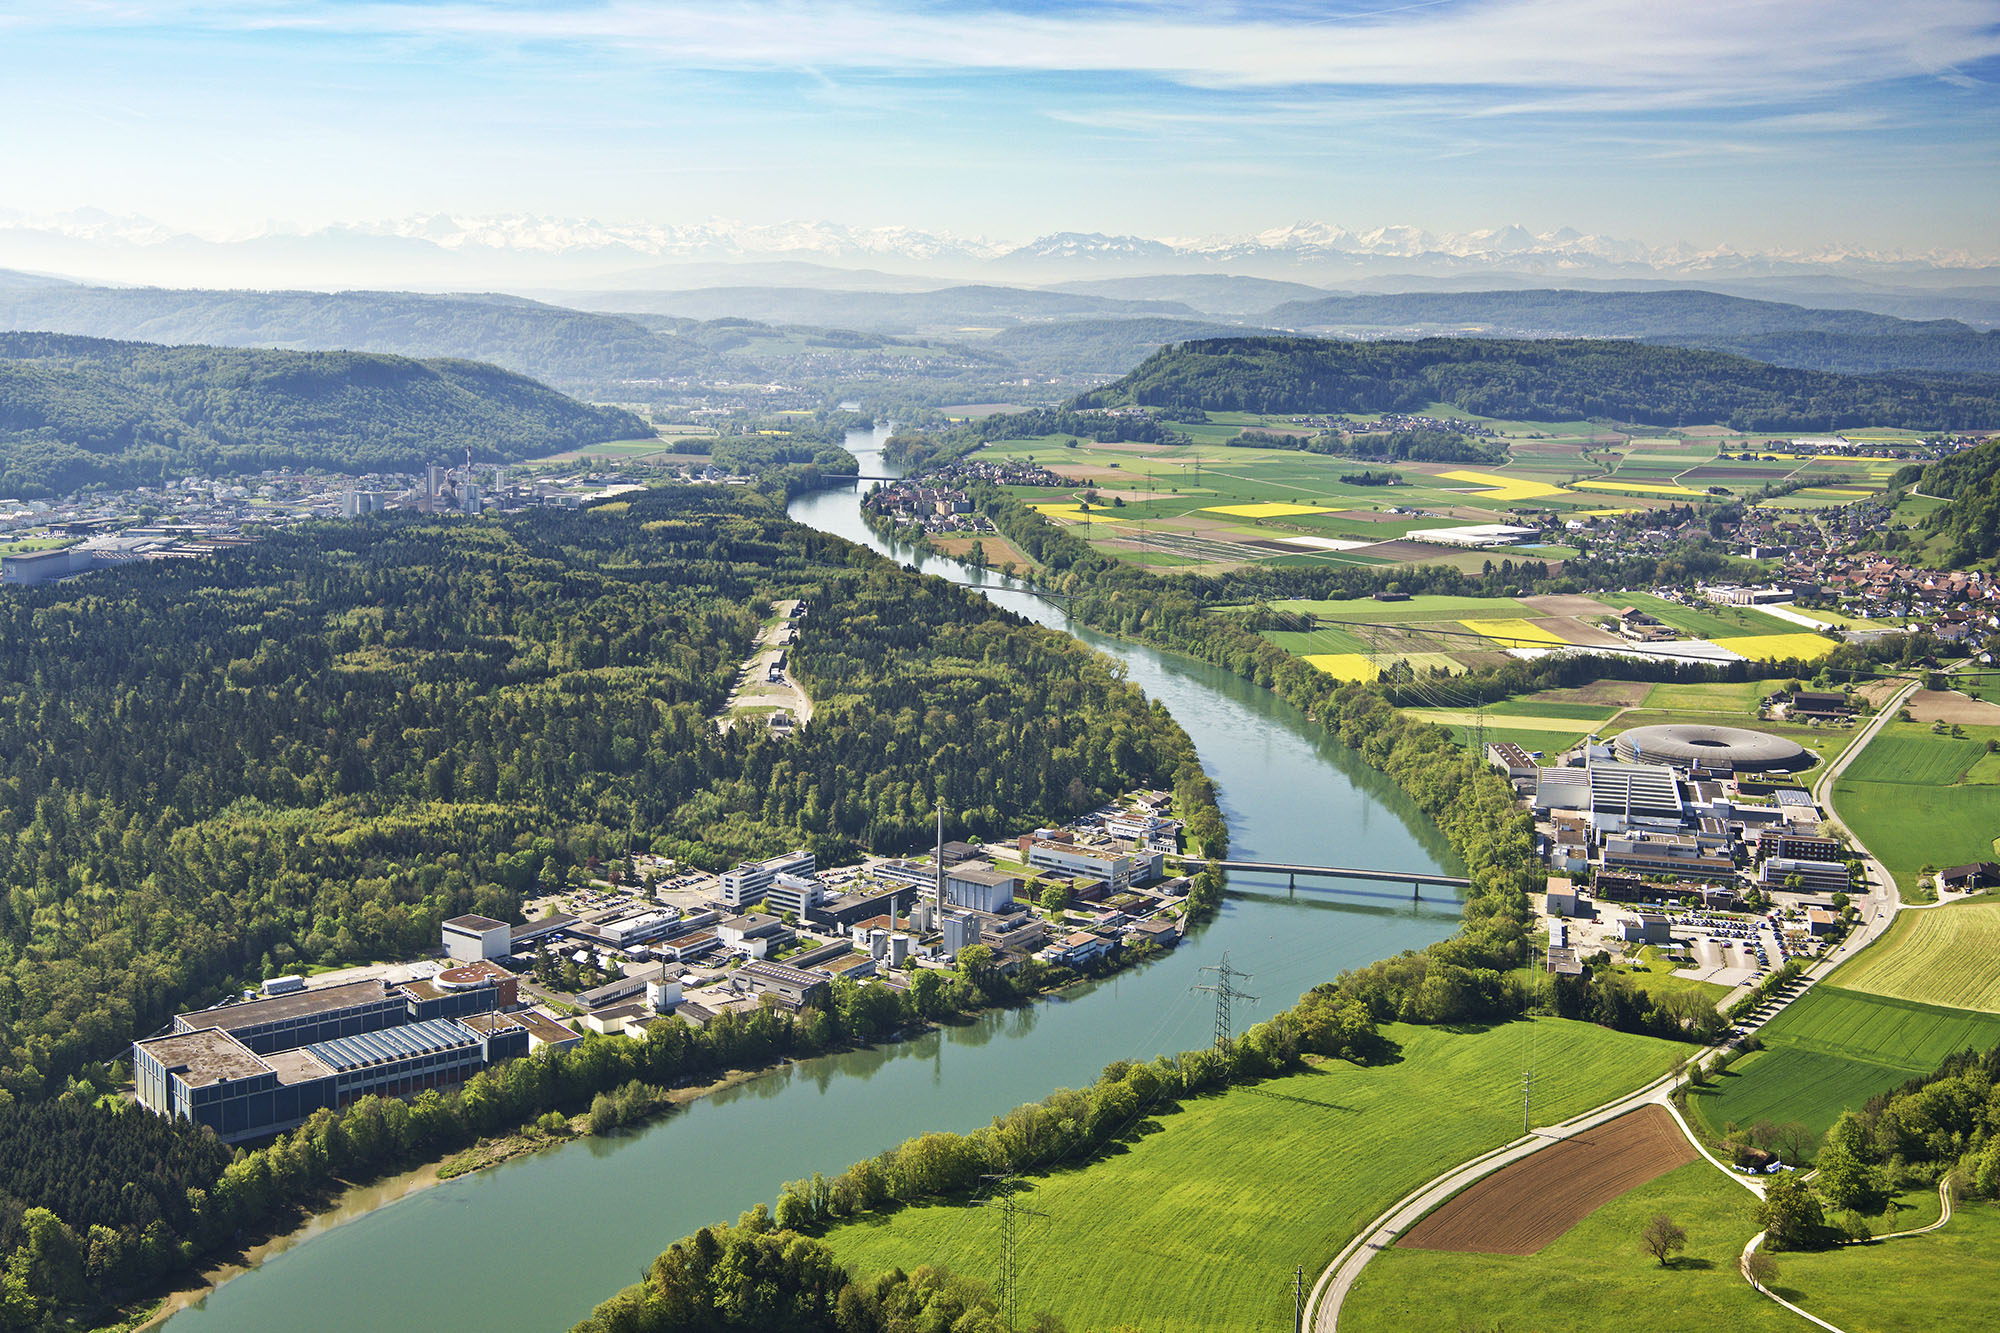
\includegraphics[height=0.5\textheight]{logos/PSI_helicopter}};
      \node [anchor=south west, inner sep = 1,fill=white, opacity=0.8] at (3.5, 0.0)
            {\tiny WIR SCHAFFEN WISSEN – HEUTE FÜR MORGEN};
    \end{tikzpicture}
    
\begin{tikzpicture}
      \filldraw[fill=lightgray!40!white, draw = none] (0,0) rectangle (1,0.5\textheight);
    \end{tikzpicture}
  \end{adjustbox}
  \vspace{0.1cm}\\
  {\usebeamerfont{subtitle} \footnotesize \insertauthor\, ::  \insertinstitute}
  \vspace{0.4cm}
  {\usebeamerfont{title} \LARGE \inserttitle}\\
  \vspace{0.4cm}
  {\usebeamerfont{subtitle} \footnotesize \insertdate}\\
  \vfilll
  \null\hfill\tiny Contact: \url{\myEmail}
\end{frame}


%----------------------------------------------------------------------------------------
%	PRESENTATION SLIDES
%----------------------------------------------------------------------------------------
\section{Progress Report}
\begin{frame}
    \frametitle{Introduction : Combining Vlasov and Fokker-Plank}


    Vlasov Equation with a Fokker Plack collisional term (\cite{Risken1984FokkerPlanckE}): \\
\vspace{1.5mm}
     \begin{equation}
         \frac{\partial f(\bm r,\bm v)}{\partial t} + \bm{v} \cdot \frac{\partial f}{\partial \bm r} + \frac{\bm{F}}{m} \cdot \frac{\partial f}{\partial \bm v} = \left(\frac{\partial f}{\partial t}\right)_{\text{coll}}
     \end{equation}

\vspace{2.5mm}

             \begin{equation}
             \left( \frac{\partial f(\bm v)}{\partial t}\right)_{\text{coll}} = -\frac{\partial}{\partial \bm{v}} \cdot (f \underbrace{\addstackgap[6pt]{\langle \Delta\mathbf{v} \rangle}}_{\bm{F_d}}) + \frac{1}{2} \frac{\partial^2}{\partial \mathbf v \partial \mathbf v} : (f \underbrace{\addstackgap[6pt]{\langle \Delta \mathbf{v} \Delta \mathbf{v^T} \rangle}}_{\bm{D}})
             \end{equation}
\vspace{3mm}

  $\bm{F_d}$ and $\bm{D}$ are approximated by Rosenbluth Potentials via following \\elliptic identities (\cite{rosenbluth}):
 \begin{align}
     \nabla_{\bm{v}}^2 \nabla_{\bm{v}}^2 G(\bm v) &=  -8 \pi f(\bm v) \\[12pt]
     \nabla_{\bm{v}}^2 G(\bm v) &= H(\bm v)
 \end{align}	

\end{frame}


\begin{frame}
    \frametitle{Resulting Langevin Scheme and Problem Setting}
Stochasticity is accounted for by  $d\bm W_t$ following $\langle d\bm W_t \rangle = 0$ and $\langle d\bm W_t d\bm W_t^T \rangle = \bm I \cdot dt$.

\begin{equation}
\left\{
 \begin{align}
	 \quad \frac{d \bm r}{dt} &= \bm v \\
	 \frac{d \bm v}{dt}  &=  \frac{\bm F}{m} + \bm F_d + \bm Q \cdot d\bm W_t \\
	 \bm D &= \bm Q \bm Q^T
 \end{align}	
\right.
\end{equation}

\vspace{3mm}

\begin{large}
    \textbf{Disorder Induced Heating (DIH):}
\end{large}

\vspace{2.5mm}

\begin{itemize}[label=$\bullet$]
     \setlength{\itemsep}{3mm}
     \item Unphysical initial condition (zero vel. particles)
     \item Cold plasma beam evolves from a disordered state to an ordered one when emitted from a electron gun
    \item The beam is heated by the disorder in the plasma
    \item Resolving collisions is thus crucial for the simulation of the beam
 \end{itemize}

\end{frame}

\begin{frame}
    \frametitle{Chainable Differential Stencils in 3D}
	 \begin{columns}
		 \column{0.50\textwidth}

\begin{itemize}[label=$\bullet$]
     \setlength{\itemsep}{3mm}
     \item Allows concatentation of any 1D user defined stencils
    \item Can define one stencil type per dimension and operator
 \end{itemize}

 \vspace{6mm}
Generalized Hessian Operator for the calculation of the Diffusion tensor $\bm{D}$
\begin{itemize}[label=$\bullet$]
     \setlength{\itemsep}{3mm}
	\item Want: FD / BD on system boundaries; centered differencing in the interior
     \item Can create separate operators for center, face, edge and slab subdomains of the 3D grid 
\end{itemize}


		 \column{0.5\textwidth}
		 \begin{figure}
			 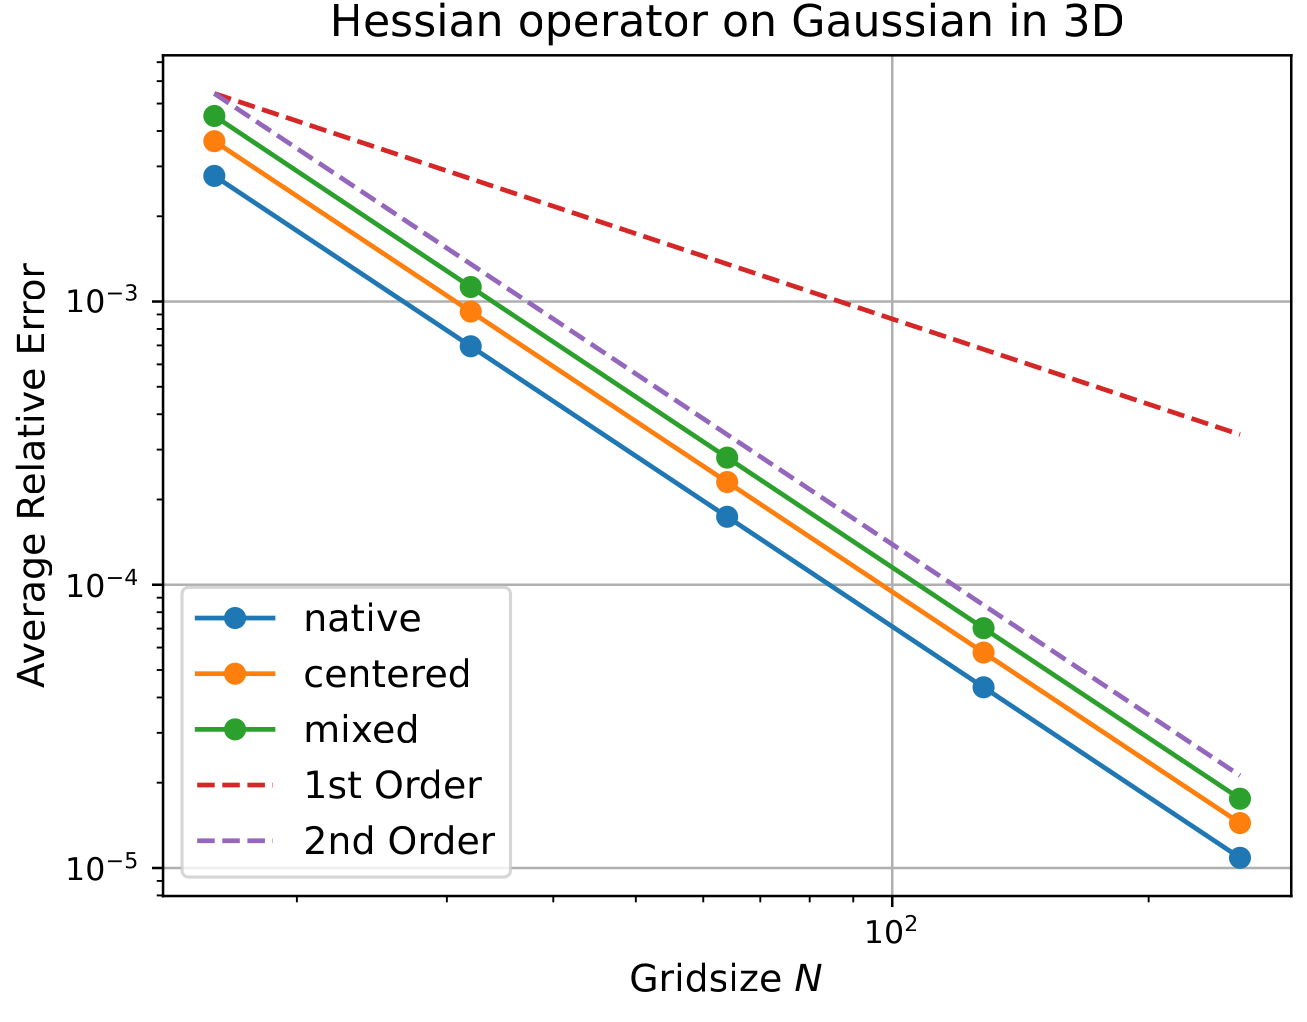
\includegraphics[scale=0.14]{figures/rel_error_hess.png}
			 \caption{Error Convergence of concatenated stencils} 
			 \label{fig:rel_error_hess}
		 \end{figure}
	 \end{columns}


\end{frame}

\begin{frame}
    \frametitle{Chainable Differential Stencils in 3D}


    Defining an operator for the second derivative: $\bm{\frac{\partial}{\partial x} \cdot \frac{\partial}{\partial x}}$
\lstinputlisting[caption=Stencil Definition, label={lst:stencils}, language=C++]{stencils.cpp}

\lstinputlisting[caption=Operator Definition, label={lst:operators}, language=C++]{operator.cpp}

\end{frame}


\begin{frame}
    \frametitle{Analysis of Current Solver (I)}

    \begin{large}
    \begin{itemize}
        \setlength{\itemsep}{6mm}
        \item[($\boldcheckmark$)] Not parallelizeable

            \begin{itemize}[label=$\bullet$]
                \setlength{\itemsep}{4mm}
                \item Some parts had to be made GPU compatible
                \item Shared memory parallelism only for collisionless solver
            \end{itemize}
\item[ \ $\boldcheckmark$\ ] Consisted of two large files of convoluted code
            \begin{itemize}[label=$\bullet$]
                \setlength{\itemsep}{4mm}
                \item Improve general readability
                \item Refactoring
                \item Split into multiple files
            \end{itemize}

    \end{itemize}
    \end{large}

\vspace{3mm}

\begin{center}
\begin{tabular}{ c c c }
 $\boldcheckmark$ : fixed  & ($\boldcheckmark$) : partially accomplished & \XSolidBrush : still problematic \\ 
\end{tabular}
\end{center}
\end{frame}

\begin{frame}
    \frametitle{Analysis of Current Solver (II)}

    \begin{large}
    \begin{itemize}
        \setlength{\itemsep}{6mm}
        \item[($\boldcheckmark$)] With collisions, crashed after a few timesteps

            \begin{itemize}[label=$\bullet$]
                \setlength{\itemsep}{6mm}
                \item Particles leave domain with FFT solver (open boundary conditions)
            \end{itemize}
\item[\ \XSolidBrush\ ] Results suggest Drag/Diffusion forces are too strong
    \begin{itemize}[label=$\bullet$]
        \setlength{\itemsep}{6mm}
        \item Current workaround: Scale each term by a tunable factor
        \item Would be cheaper to compute collisions every $n$-th timestep (\cite{stoel})
    \end{itemize}

    \end{itemize}
    \end{large}

        \vfill
\begin{center}
\begin{tabular}{ c c c }
 $\boldcheckmark$ : fixed  & ($\boldcheckmark$) : partially accomplished & \XSolidBrush : still problematic \\ 
\end{tabular}
\end{center}

\end{frame}

\begin{frame}
    \frametitle{Analysis of Current Solver (III)}
    \begin{large}
    \begin{itemize}
        \setlength{\itemsep}{6mm}
        \item[($\boldcheckmark$)] Results only stable for considered time frame (5 plasma periods)

            \begin{itemize}[label=$\bullet$]
                \setlength{\itemsep}{4mm}
                \item Apparent upward trend for longer time frames (see next slide)
            \end{itemize}
\item[\ \XSolidBrush\ ] High memory consumption for $256^3$ spatial grid (use Kokkos functionality for profiling)
    \begin{itemize}[label=$\bullet$]
                \setlength{\itemsep}{4mm}
                \item Some fields could be shared (i.e. currently storing 17 Scalar fields;\\ not counting temp. fields of the 3 FFT solvers!)
            \end{itemize}

    \end{itemize}
    \end{large}

        \vfill
\begin{center}
\begin{tabular}{ c c c }
 $\boldcheckmark$ : fixed  & ($\boldcheckmark$) : partially accomplished & \XSolidBrush : still problematic \\ 
\end{tabular}
\end{center}

\end{frame}

\begin{frame}
    \frametitle{Comparison to P3M}

     Change in mesh size drastically improves results, though an upwards trend becomes apparent:

\begin{figure}[!htb]
%\minipage{0.65\textwidth}%
  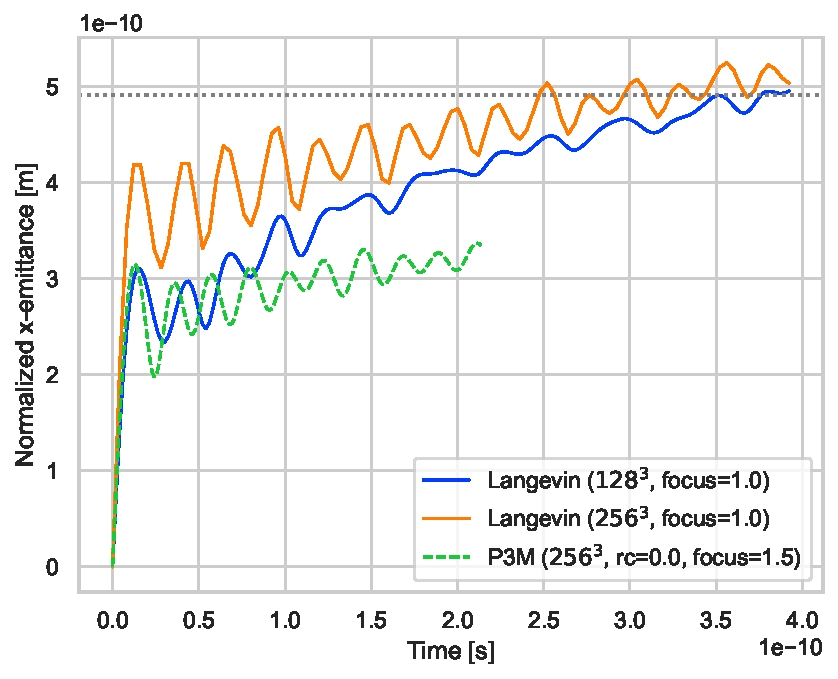
\includegraphics[width=0.5\linewidth]{figures/comparison_meshsize.pdf}
    \caption{Normalized Emittance of a cold sphere w/o collisions} 
  \label{fig:awesome_image3}
%\endminipage
\end{figure}

\end{frame}

\begin{frame}
    \frametitle{Comparison to P3M}

     \item Constant focusing factor is an important hyperparameter:
     \begin{columns}
         \column{0.50\textwidth}

\begin{figure}[!htb]
%\minipage{0.65\textwidth}%
  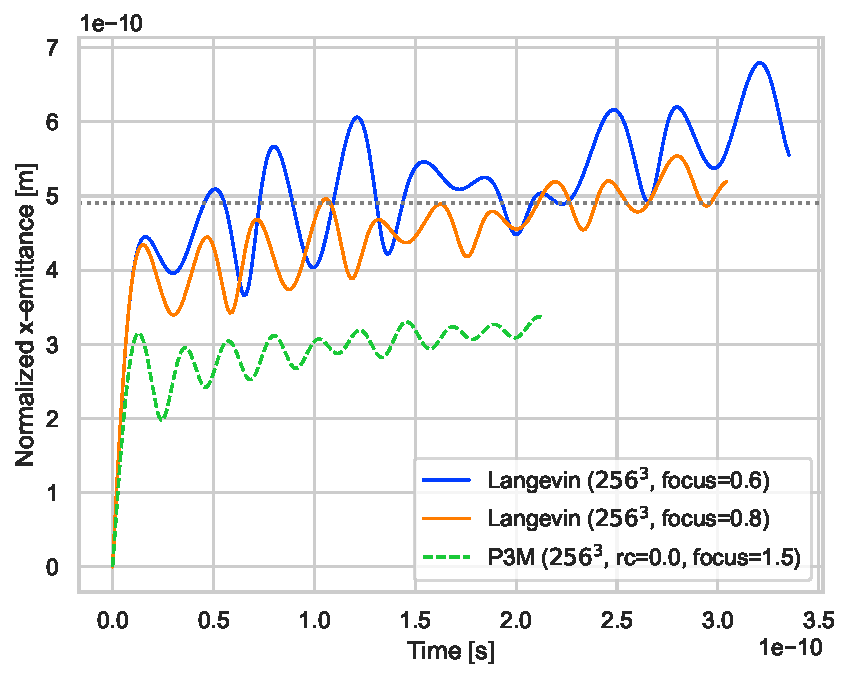
\includegraphics[width=0.9\linewidth]{figures/comparison_low_focus.pdf}
    \caption{Decreased Constant Focusing} 
  \label{fig:awesome_image3}
%\endminipage
\end{figure}

         \column{0.50\textwidth}
\begin{figure}[!htb]
%\minipage{0.65\textwidth}%
  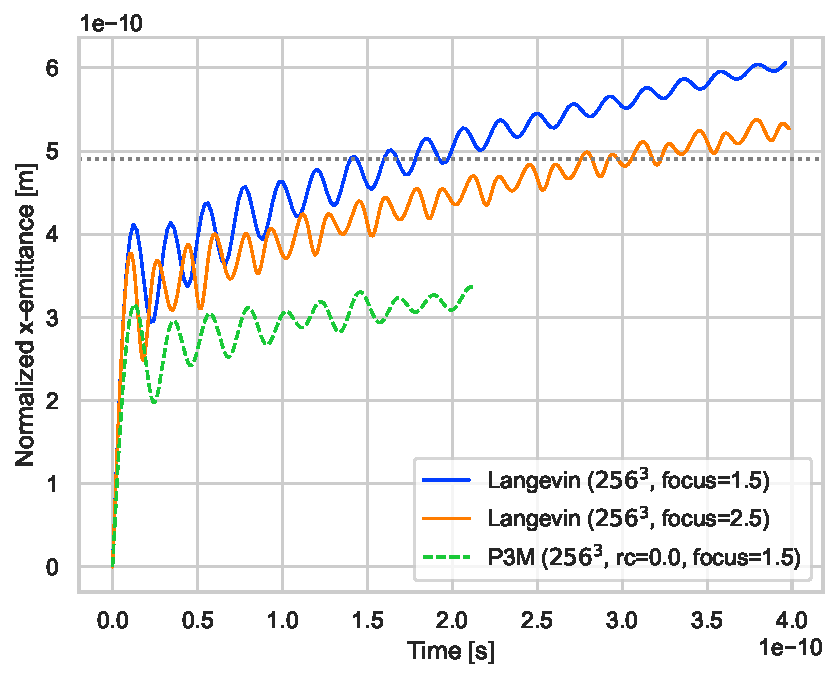
\includegraphics[width=0.9\linewidth]{figures/comparison_high_focus.pdf}
    \caption{Increased Constant Focusing} 
  \label{fig:awesome_image3}
%\endminipage
\end{figure}

     \end{columns}

\end{frame}

\section{Timeline}

\begin{frame}
\frametitle{Timeline in Restrospect}
\begin{table}[]
\def\arraystretch{1.5}
\begin{tabular}{p{0.08\linewidth} | p{0.85\linewidth}}
Date & Target Goals \\
\hline \hline
30/01 & Assist Severin and ensure correctness of current implementation \\
20/02 & \sout{Find Order of convergence / accuracy} and compare whether really much better than P3M (even though it might still run only on single core) \\
20/02 & \textcolor{gray}{Ensure Performance Portability (MPI, OpenMP and GPU)} \\
06/03 & Benchmarking of \sout{accuracy}, \textcolor{gray}{runtime} and \sout{scalability} \\
27/03 & \textcolor{gray}{Start improving most pressing bottlenecks} \\
\end{tabular}
\caption{Initial Timeline; Font-Encoding: \textcolor{gray}{partially accomplished}, \sout{not accomplished} }
\end{table}

\end{frame}

\begin{frame}
\frametitle{Timeline Going Forward}

\begin{table}[]
\def\arraystretch{1.5}
\begin{tabular}{p{0.08\linewidth} | p{0.85\linewidth}}
Date & Target Goals \\
\hline \hline
08/05 & Find causes of divergence / phase shift in comparison to P3M \\
      & Carry out rigorous profiling \\
      & Analyse Friction / Diffusion coefficients \\
08/05 & Implement algorithmic improvements and compare accuracy / performance to previous implementation \\
12/06 & Start writing and code clean-up \\
03/07 & Submission \\
\end{tabular}
\caption{Timeline with approximate milestones}
\end{table}

\end{frame}

\begin{frame}
    \frametitle{Conclusion}

\begin{itemize}[label=$\bullet$]
     \setlength{\itemsep}{3mm}
     \item Implementation of Generalized Hessian Operator
     \item Refactoring and verification of Severin's results
     \item Comparison to P3M (observation of unphysical upward trend)
 \end{itemize}
 \vspace{5mm}

 Personal Take-Aways:

\begin{itemize}[label=$\bullet$]
     \setlength{\itemsep}{3mm}
     \item Don't loose yourself in small details
     \item Actively seek discussions about the current problems with supervisors and students
     \item Keep an eye on the timeline, adjust if necessary
 \end{itemize}

\end{frame}

 \begin{frame}[allowframebreaks]
     \frametitle{References}
     \bibliographystyle{apalike}
     \bibliography{references.bib}
 \end{frame}


 \begin{frame}
 \frametitle{Rosenbluth Potentials \cite{rosenbluth}}

	 \begin{columns}[t] 
		 \begin{column}{0.5\textwidth}
 Potentials on velocity space only \cite{PlasmaKineticTheory}:
 \begin{align}
	 \Gamma   &= \frac{q^4 \ln(\Lambda)}{4 \pi \epsilon_0^2 m^2} \\[9pt]
	 H(\bm v) &=  2 \int d^3 v^\prime \frac{f(\bm{v^\prime})}{|\bm v - \bm{v^\prime}|} \\[9pt]
	 G(\bm v) &=  \int d^3 v^\prime f(\bm{v^\prime}) |\bm v - \bm{v^\prime}| \\[9pt]
	 \langle \Delta\mathbf{v} \rangle &=  \Gamma \frac{\partial H}{\partial \bm v} = \bm{F_d} \\[9pt]
	 \langle \Delta\mathbf{v}\Delta\mathbf{v}^T \rangle &=  \Gamma \frac{\partial^2 G}{\partial \bm v \partial \bm v} = \bm D
 \end{align}	
 \end{column}
 \hspace{-8pt}
 \vrule{}
 \hspace{+7pt}
		 \begin{column}{0.4\textwidth}
 Resulting Elliptic Identities: \\[6pt]
 \begin{align}
	 \nabla_{\bm{v}}^2 \nabla_{\bm{v}}^2 G(\bm v) &=  -8 \pi f(\bm v) \\[21pt]
	 \nabla_{\bm{v}}^2 G(\bm v) &= H(\bm v)
 \end{align}	
 \end{column}
\end{columns}

 \end{frame}
%\begin{frame}
    %\frametitle{Periodic Poisson Solver}

%\begin{figure}[!htb]
%\minipage{0.33\textwidth}
  %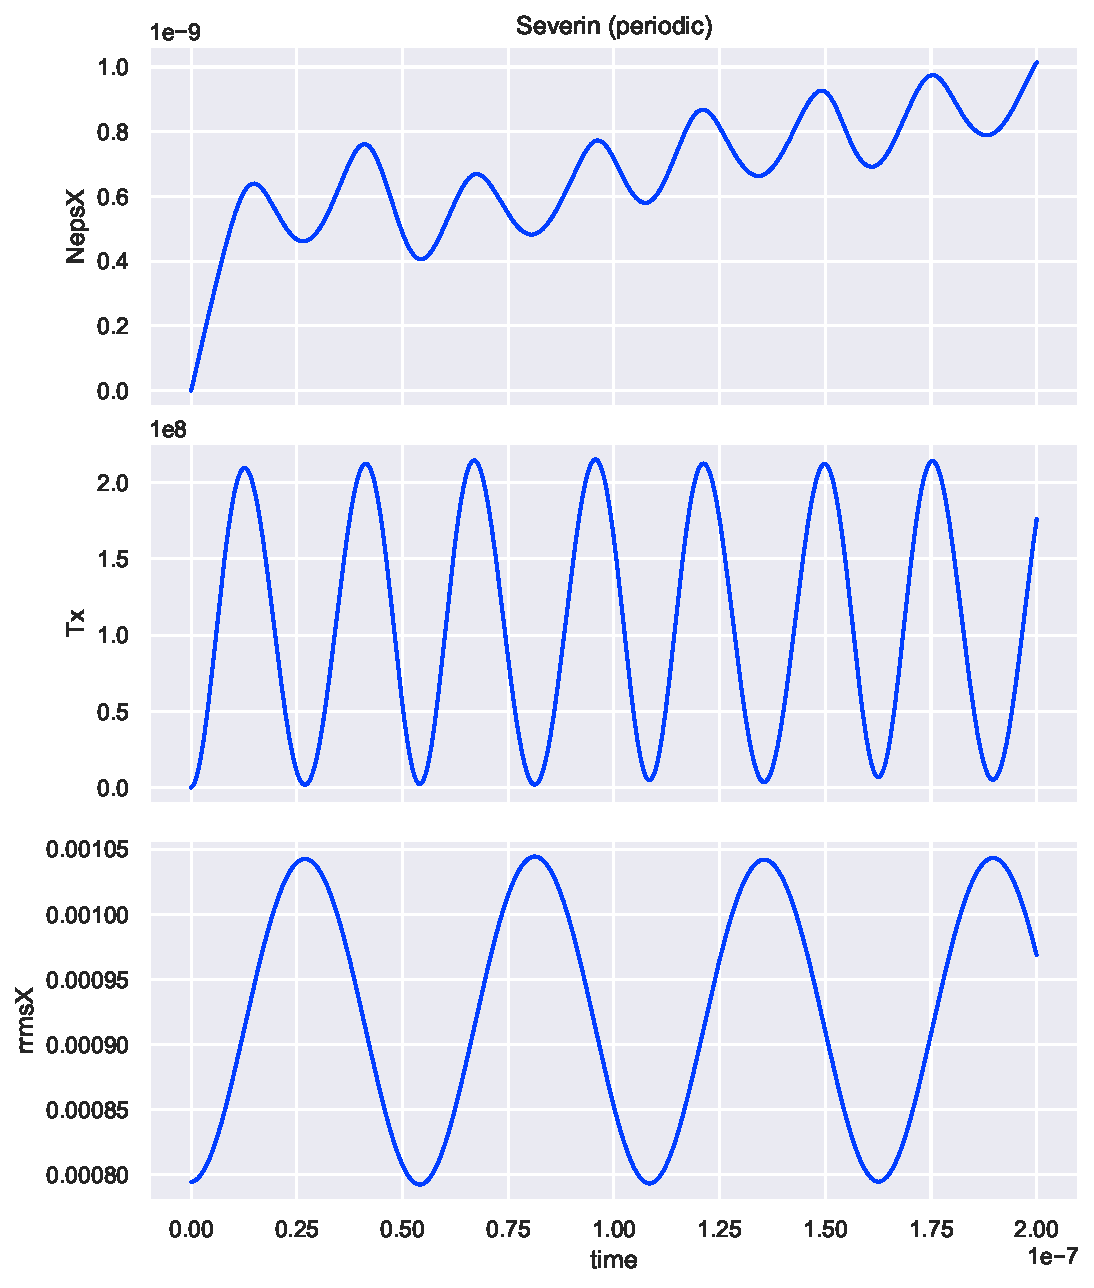
\includegraphics[width=1.1\linewidth]{figures/severin_vanilla_periodic.pdf}
  %\label{fig:awesome_image2}
%\endminipage\hfill
%\minipage{0.33\textwidth}%
  %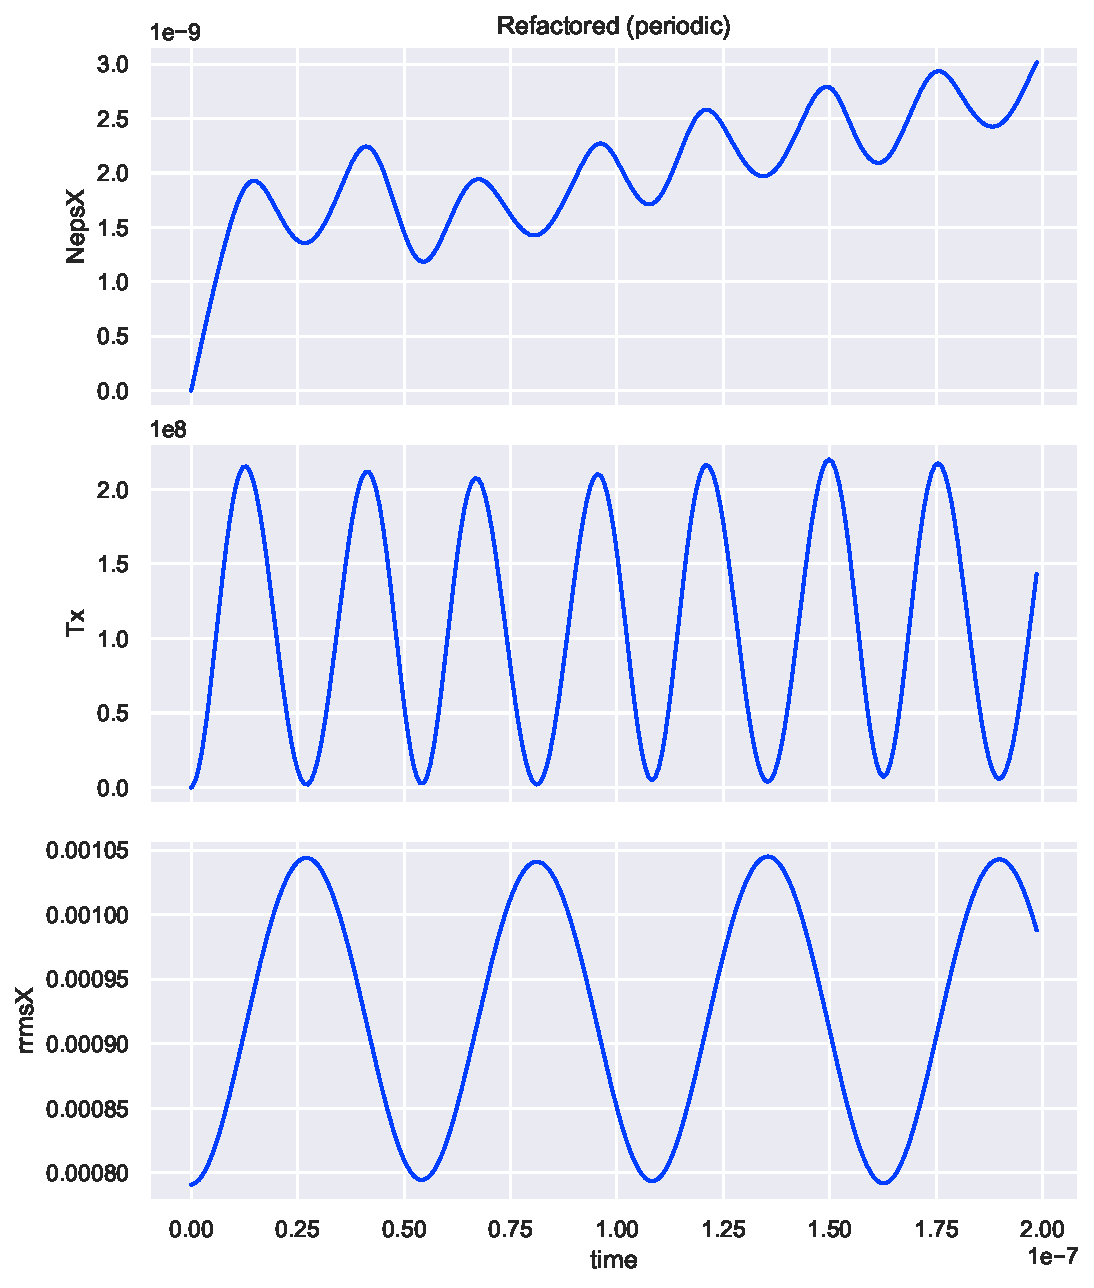
\includegraphics[width=1.1\linewidth]{figures/refactored_periodic.pdf}
  %\label{fig:awesome_image3}
%\endminipage
%\minipage{0.33\textwidth}%
  %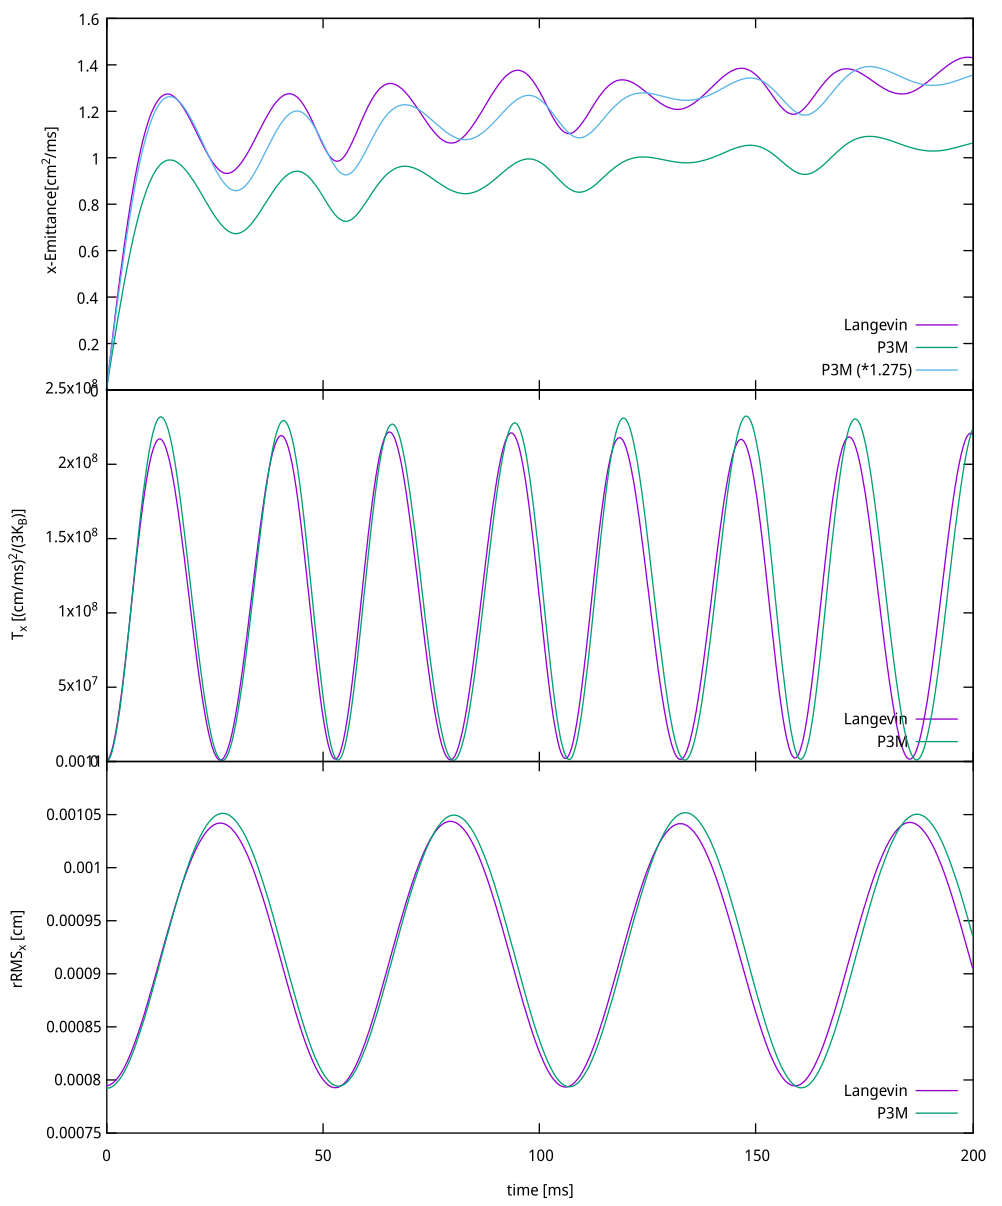
\includegraphics[width=1.1\linewidth]{figures/thesis_plot.png}
  %\label{fig:awesome_image3}
%\endminipage
%\end{figure}

%\end{frame}

%\begin{frame}
    %\frametitle{Investigating the Focus Force}

%\begin{figure}[!htb]
%\minipage{0.40\textwidth}%
  %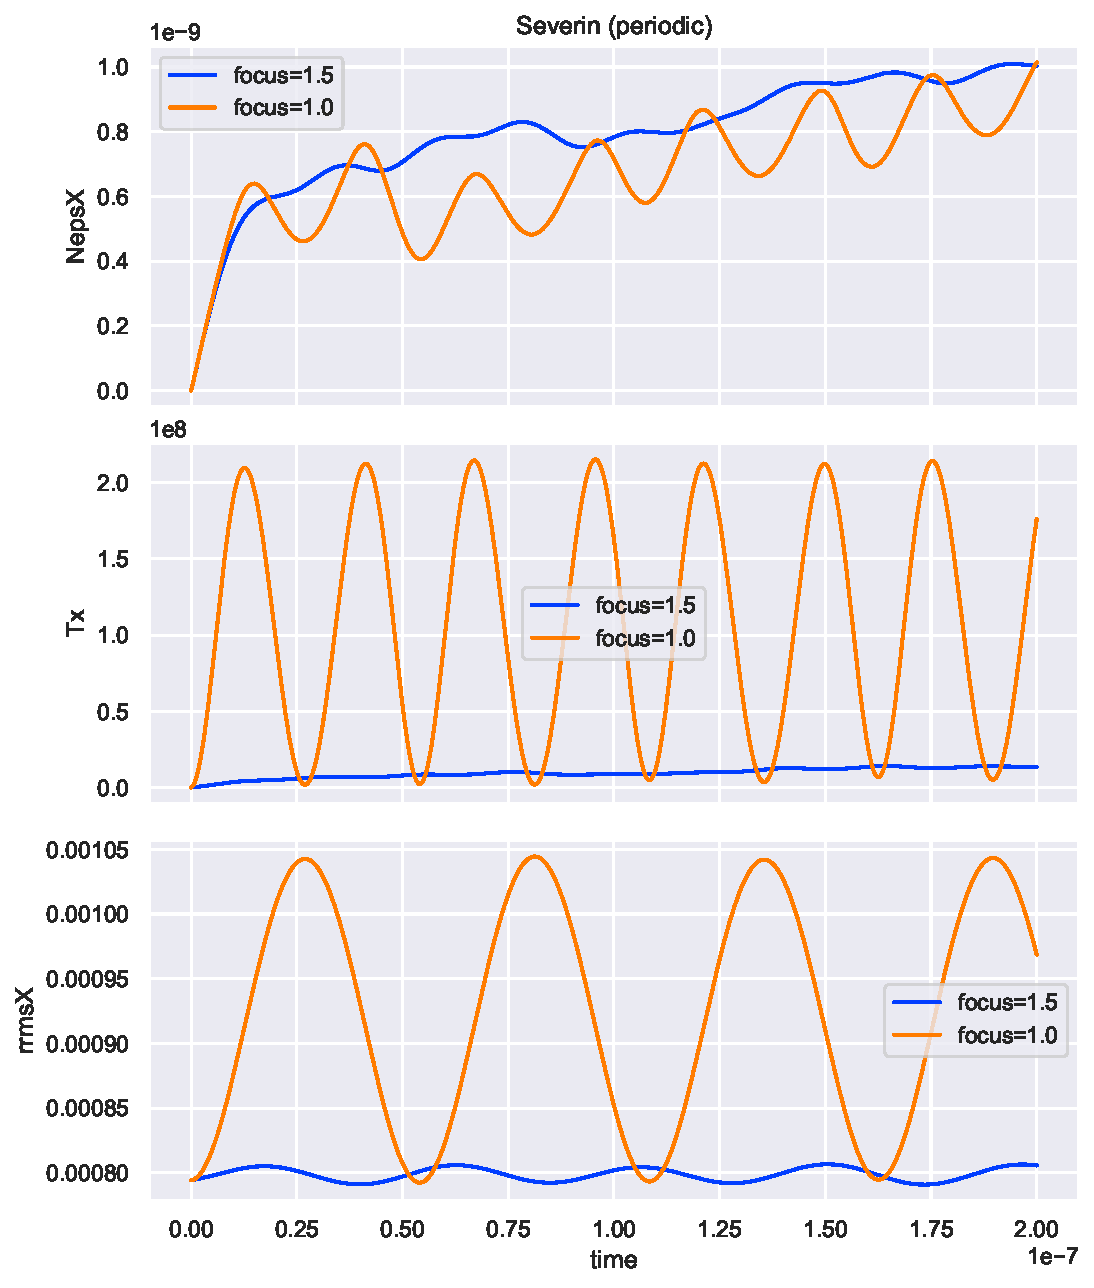
\includegraphics[width=1.1\linewidth]{figures/focus_comparison.pdf}
  %\label{fig:awesome_image3}
%\endminipage
%\end{figure}

%\end{frame}

%\begin{frame}
    %\frametitle{Conclusion about Results}

%\begin{itemize}[label=$\bullet$]
    %\item Emittance increases with time
	%\item Emittance is far too small as compared to Severin's results
    %\item Results in Severin's Thesis possibly are made with open b.c. Solver
%\end{itemize}

%\end{frame}

%\begin{frame}
    %\frametitle{How to proceed}

%\begin{itemize}[label=$\bullet$]
    %\item Continue with super-cell approach (not copying anything from Severin's code)
	%\item Different formula for constant focusing?
    %\item Reformulate Thesis goals!
	%\item More regular discussions with Sonali / Sri
%\end{itemize}

%\end{frame}


%\section{Motivation for High-Dimensional UQ: Example from Nuclear Physics}
%\frame[noframenumbering]{\tableofcontents[currentsection]}

%\begin{frame}
  %\frametitlepsi{Definition of Uncertainty Quantification (UQ)}

  %\Large
  %Uncertainty Quantification (UQ) aims to calculate the effect of unknown or uncertain system parameters on the outcome of an experiment or computation.
%\end{frame}
  
%\begin{frame}
  %\frametitlepsi{Definition of Uncertainty Quantification (UQ)}
  
  %Let $f\in L^2(\mathbb{R}^d)$ be a \textbf{computationally expensive} model with 

  %\begin{equation*}
    %f\colon \begin{array}[t]{ >{\displaystyle}r >{{}}c<{{}}  >{\displaystyle}l } 
          %\mathbb{R}^{d} &\to& \mathbb{R} \\ 
          %\mvec x &\mapsto& f(\mvec x)\,.
         %\end{array}
  %\end{equation*}
  %Let $\mvec x = (x_1,x_2,...,x_d)$ be an input with uncertainty $\Delta\mvec x$. \\
  %What is the uncertainty in $f(\mvec x)$?
  
  %\vspace{1cm}

  %\onslide<2->{
    %Common approach, model input as random variable $\mvec X\sim\mathcal{N}(\mvec x, \Sigma)$, with $\Sigma\in\mathbb{R}^{d\times d}$ the covariance matrix (uncertainties and correlations):
    
        %\begin{center}
      %% Flowchart MC UQ
      %\begin{tikzpicture}[node distance = 3.5cm, auto]
        %\tikzstyle{block} = [rectangle, draw, fill=white, 
          %text width=10em, text centered, rounded corners, minimum height=4em]
        
        %% \tikzstyle{line} = [draw, -latex']
        %\tikzstyle{line} = [draw, -{Triangle[scale=2]}]
        
        %\node [block, text width=8em] (1) {
          %$X\sim\mathcal{N}(\vec x,\Sigma)$
          %\includegraphics[width=\textwidth]{plots/posterPlot-SUQ-input}
        %};
        %\node [block, right of=1, text width=8em] (2) {
          %$f(X)$
          %\includegraphics[trim={0 43 0 0}, clip, width=\textwidth]{plots/posterPlot-SUQ-output_v3}
        %};

        %\path [line] (1) -> (2);
      %\end{tikzpicture}
    %\end{center}
  %}

  %\onslide<3->{
    %Concentrate on \textit{Response Variability Methods}: estimate mean and variance of output
    %\[f(\mvec x) = \mu \pm \sigma\,.\]
  %}
  
%\end{frame}

%\begin{frame}
  %\frametitlepsi{Motivation: SNF Characterisation}

  %\onslide<-2>{
    %Nuclear burnup simulations are used to characterise spent nuclear fuel:
    %{
      %\large
      %\begin{equation*}
        %f:\underbrace{
          %\begin{pmatrix}
            %\texttt{Fresh fuel parameters} \\
            %\texttt{Irradiation history} \\
            %\texttt{Reactor parameters}\\
            %\texttt{Nuclear Data}
          %\end{pmatrix}
        %}_{
          %\text{Input with known uncertainty}
        %}
        %\rightarrow
        %\underbrace{
          %\begin{pmatrix}
            %\texttt{Decay Heat} \\
            %\texttt{Isotopic Content}\\
            %\texttt{Criticality}
          %\end{pmatrix}
        %}_{
          %\text{Output with unknown uncertainty}
        %}
      %\end{equation*}
    %}
  %}
  %\onslide<3->{
    %\begin{equation*}
      %\begin{split}
        %f:\mathbb{R}^{15000}&\rightarrow\mathbb{R}\\
        %\text{Nuclear Data}&\rightarrow\text{Decay Heat}
      %\end{split}
    %\end{equation*}
  %}

  %Any uncertainty in outputs will increase the risks and costs of 
  %\begin{figure}
    %\centering
    %\includegraphics[width=0.25\textwidth]{img/transport.PNG}
    %\includegraphics[width=0.25\textwidth]{img/storage.PNG}
    %\includegraphics[width=0.25\textwidth]{img/disposal.PNG}
    %\caption{\large Transport \hspace{1.8cm} Storage \hspace{1.8cm} Disposal}
  %\end{figure}

  %\onslide<2->{
    %\Large
    %\textbf{Accurate estimation of uncertainty saves money and reduces risks.}
  %}

%\end{frame}

%\subsection{Current Methods and Shortcomings}
%\subsubsection{Simple MC}
%\subsubsection{Surrogate Models}
%\frame[noframenumbering]{\tableofcontents[currentsection]}

%\begin{frame}
  %\frametitlepsi{
    %Simple Monte Carlo UQ}

  %\begin{enumerate}[label*=\arabic*.]
  %\item $\quad$
    %\vspace{-1cm}
    %\begin{center}
      %% Flowchart MC UQ
      %\begin{tikzpicture}[node distance = 3.5cm, auto]
        %\tikzstyle{block} = [rectangle, draw, fill=blue!20, 
          %text width=10em, text centered, rounded corners, minimum height=4em]
        
        %% \tikzstyle{line} = [draw, -latex']
        %\tikzstyle{line} = [draw, -{Triangle[scale=2]}]
        
        %\node [block] (1) {
          %Sample inputs $\vec x_1,...,\vec x_N\sim\mathcal{N}(\vec x,\Sigma)$
          %\includegraphics[width=\textwidth]{plots/posterPlot-SUQ-input}
        %};
        %\node [block, right of=1, text width=6em] (2) {
          %Run $f(\vec x_i)$ $N$ times
        %};
        %\node [block, right of=2, text width=12em] (3) {
          %Compute sample mean and variance\\
          %\includegraphics[width=\textwidth]{plots/posterPlot-SUQ-output_v3}
        %};

        %\path [line] (1) -> (2);
        %\path [line] (2) -> (3);
      %\end{tikzpicture}
    %\end{center}

    %\item Compute sample mean and variance
    %\begin{equation*}
      %\mu_N = \frac{1}{N}\sum_{i=1}^N f(\mvec x_i)\,,\quad\sigma^2_N = \frac{1}{N-1}\sum_{i=1}^N \left(f(\mvec x_i) - \sum_{j=1}^N \frac{f(\mvec x_j)}{N}\right)^2\,.
    %\end{equation*}

  %\end{enumerate}
  %\onslide<2->{
    %Simple MC is unbiased, but slow (error$=\sqrt{\MSE}=\bigO\left(\frac{1}{\sqrt{N}}\right)$):
    %\begin{align*}
      %\lim_{N\rightarrow\infty}\mu_N = \E[f]\,,& \quad\text{since }\MSE\Big(\mu_N-\E[f]\Big) = \frac{\Var[f]}{N}\,,\\
      %\lim_{N\rightarrow\infty}\sigma^2_N = \Var[f]\,,& \quad\text{since }\MSE\Big(\sigma^2_N - \Var[f]\Big) = \frac{1}{N}\left(m_4[f] - \frac{N-3}{N-1}{\Var}^2[f]\right)\,.
    %\end{align*}
  %}
%\end{frame}

%\begin{frame}
  %\frametitlepsi{Simple Monte Carlo UQ}

  %Simple MC is the current approach used for nuclear data propagation:
  %\begin{itemize}[label=--]
  %\item MC converges as $\bigO\left(\frac{1}{\sqrt{N}}\right)$, i.e. many simulations required!
  %\item E.g. for SNF characterisation $N\sim 1000$, with each simulation lasting a few hours.
  %\item Expecting $>12000$ fuel assemblies in Switzerland.
  %\item $\Rightarrow$ millions of CPU hours  $\Rightarrow$ \textbf{MC UQ is too slow!}
  %\end{itemize}
%\end{frame}

%\begin{frame}
  %\large
  %In summary: simple MC and surrogate models are inadequate for high-dimensional UQ.
%\end{frame}


%\section{New method: Lasso Monte Carlo}
%\subsection{Multilevel Monte Carlo}
%\subsection{Lasso Regression}
%\frame[noframenumbering]{\tableofcontents[currentsection]}

%\begin{frame}
  %\frametitlepsi{Lasso Monte Carlo}
  %\large
  %Lasso Monte Carlo (LMC) is a new technique that combines two existing methods:
  %\begin{itemize}[label=--]
  %\item Multilevel Monte Carlo (MLMC) \citep{giles_multilevel_2008, krumscheid_quantifying_2020}
  %\item Lasso regression \citep{tibshirani_regression_1996}
  %\end{itemize}

%\end{frame}

%\begin{frame}
  %\frametitlepsi{MLMC}
  %MLMC combines models of different levels of fidelity.

  %\vspace{.5cm}
  %Let $X$ be a random variable, and $f_1,f_2,..., f_L$ be models of increasing accuracy, and increasing computational cost. Then
  %\begin{equation*}
    %\mathbb{E}[f_L(X)] = \mathbb{E}[f_1(X)] + \mathbb{E}[f_2(X) - f_1(X)] + \mathbb{E}[f_3(X) - f_2(X)] + ... + \mathbb{E}[f_{L-1}(X) - f_L(X)]
  %\end{equation*}

  %\onslide<2->{
    %Terms computed with
    %\begin{equation*}
      %\mathbb{E}[f_\ell(X) - f_{\ell-1}(X)] = \frac{1}{N_\ell}\sum_{i=1}^{N_\ell}\{f_\ell(x_i)-f_{\ell-1}(x_i)\},
    %\end{equation*}
    %will converge as $\mathcal{O}\left(\frac{\Var[f_\ell - f_{\ell-1}]}{\sqrt{N_L}}\right)$.
  %}
  
  %\onslide<3->{
    %So if we have
    %\begin{equation*}
      %\Var(f_1) > \Var(f_2-f_1) > \Var(f_3-f_2) > ... > \Var(f_L-f_{L-1}),
    %\end{equation*}
    
    %we require
    %\begin{equation*}
      %N_1 > N_2 > ... > N_L.
    %\end{equation*}
    
    %Overall computational cost is reduced if $N_\ell$ are correctly chosen!
  %}

  %\onslide<4->{
    %Thanks to more recent papers %\cite{bierig_estimation_2016, krumscheid_quantifying_2020}, MLMC can be used for higher order moments.
  %}
%\end{frame}

%\begin{frame}
  %\frametitlepsi{Two-level MC}
  
  %Let
  %\begin{itemize}[label=--]
  %\item $f$ be the true, expensive model, that we evaluate $N$ times: $f(\mvec x_1), f(\mvec x_2),..., f(\mvec x_{N})$.
  %\item $\widetilde f$ a cheap, biased, surrogate model, that we evaluate $N+M$ times, with $M\gg N$:  $\widetilde f(\mvec x_1), \widetilde f(\mvec x_2), ..., \widetilde f(\mvec x_{N})$, and  $\widetilde f(\mvec z_1), \widetilde f(\mvec z_2), ..., \widetilde f(\mvec z_{M})$.
  %\end{itemize}

  %\onslide<2->{
    %Then the estimators are
    %\begin{align*}
      %\mu_{N,M} &= \frac{1}{M}\sum_{i=1}^{M} \widetilde f(\mvec z_i) + \frac{1}{N}\sum_{i=1}^N f(\mvec x_i) - \widetilde f(\mvec x_i) = \widetilde\mu_M + \mu_N - \widetilde\mu_N\,,\\
      %\sigma^2_{N,M} &= \widetilde \sigma^{2}_{M} + \sigma^{2}_{N} - \widetilde \sigma^{2}_N\,.
    %\end{align*}
  %}

  %\onslide<3->{
    %\begin{itemize}[label=--]
    %\item Estimators are unbiased $\lim_{\substack{N\rightarrow\infty\\ M\rightarrow\infty}}\mu_{N,M} = \E[f]\,,\quad\lim_{\substack{N\rightarrow\infty\\ M\rightarrow\infty}}\sigma^2_{N,M} = \Var[f]\,.$
    %\item More accurate than simple MC $\mu_{N},\sigma^2_{N}$, if and only if following conditions are satisfied
      %{\small
        %\begin{align}
            %&\Var[f-\widetilde f] \leq ~\Var[f]\,,\label{eq:cond_a}\\
          %&\resizebox{1.0\hsize}{!}{$m_{2,2}\left[f+\widetilde f, f-\widetilde f\right] + \frac{1}{N-1}\Var[f+\widetilde f]\Var[f-\widetilde f] - \frac{N-2}{N-1}\left(\Var[f]-\Var[\widetilde f]\right)^2 \leq ~ m_4[f] - \frac{N-3}{N-1}{\Var}^2[f]\,.$} \label{eq:cond_b}
        %\end{align}
      %}
    %\end{itemize}
  %}

%\end{frame}

%\begin{frame}
  %\frametitlepsi{Two-level MC}
  %\large
  %Common usage of MLMC:
  %\begin{enumerate}[label*=\arabic*.]
  %\item Gather a training set $\mvec x_1, f(\mvec x_1)$, $\mvec x_2, f(\mvec x_2)$, ..., $\mvec x_{N_{tr}}, f(\mvec x_{N_{tr}})$.
  %\item Train a surrogate model $\widetilde f\sim f$, that is \textbf{fast to evaluate}.
  %\item Evaluate $\widetilde f$ $N+M$ times to obtain $\widetilde f(\mvec x_1), \widetilde f(\mvec x_2), ..., \widetilde f(\mvec x_{N})$, and  $\widetilde f(\mvec z_1), \widetilde f(\mvec z_2), ..., \widetilde f(\mvec z_{M})$.
  %\item Evaluate $f$ $N$ times, to obtain $f(\mvec x_1), f(\mvec x_2),..., f(\mvec x_{N})$.
  %\item Compute 2-level estimators $\mu_{N,M}, \sigma^2_{N,M}$.
  %\end{enumerate}

  %\vspace{1cm}

  %\onslide<2->{
    %\begin{itemize}[label=--]
    %\item Unbiased.
    %\item More accurate than simple MC for a given $N$ (if conditions (\ref{eq:cond_a}, \ref{eq:cond_b})).
    %\item However, bottleneck is still generating the training set $N_{tr}$ (especially in high-dimensional cases).
    %\end{itemize}
  %}
  
%\end{frame}

%\begin{frame}
  %\frametitlepsi{Choosing Surrogate Model}
  %\large
  %How to choose a surrogate model that satisfies convergence conditions, and can be trained with a small training set $N_{tr}\ll d$?

  %\vspace{.5cm}
  %\onslide<2->{
    %Lasso regression technique fits a sparse linear model:
    %\begin{equation*}
      %\widetilde f(\mvec x) = \mvec\beta\cdot\mvec x,\quad \text{with }\mvec\beta\text{ sparse,}
    %\end{equation*}

    %by minimising loss function
    %\begin{equation*}
      %\mathcal{L}(\mvec\beta) = \underbrace{\frac{1}{2}\sum_{i=1}^{N_{tr}}\left(f(\mvec x_i) - \mvec\beta\cdot\mvec x_i \right)^2}_{\text{OLS loss}} + \underbrace{\lambda||\mvec{\beta}||_1}_{\text{Regularisation term}}\,,
    %\end{equation*}

    %with $\lambda>0$ a chosen regularisation constant.
  %}

  %\onslide<3->{
    %\begin{itemize}[label=--]
    %\item Lasso can be trained for small training sets, without overfitting.
    %\item Does it satisfy the convergence conditions (\ref{eq:cond_a}, \ref{eq:cond_b})?
    %\end{itemize}

    %}

  
%\end{frame}

%\begin{frame}
  %\frametitlepsi{Choosing Surrogate Model}
  %\large
  
  %Does Lasso $\widetilde f$ satisfy the convergence conditions (\ref{eq:cond_a}, \ref{eq:cond_b})?

    %%%   \item Lasso satisfies convergence conditions (under some conditions on $f$), i.e. if $\widetilde f$ is a Lasso model, $\mu_{N,M},\sigma_{N,M}$ will be equally or more accurate than simple MC $\mu_N,\sigma_N$.

  %Condition \eqref{eq:cond_b}, is unfortunately not guaranteed.

  %\vspace{1cm}
  %\onslide<2->{
    %However, if $f$ is a \textit{noisy linear function}
    %\[f(\mvec x) = \mvec \alpha\cdot\mvec x + \Epsilon\,,\quad\text{with} \Epsilon\sim\mathcal{N}(0,\varepsilon)\]

    %then condition \eqref{eq:cond_b} is guaranteed! This is true to first order for any $f$:
    %\[f(\mvec x + \delta\mvec x) = f(\mvec x_0) + \delta\mvec x\cdot\mvec\nabla f(\mvec x_0) + \mathcal{O}\left(||\delta\mvec x||^2\right).\]
  %}

  %\onslide<3->{
    %I.e. the two-level estimator $\sigma^2_{N,M}$ with Lasso, will often converge faster than simple MC, and is guaranteed to do so under certain conditions on $f$.
  %}
  
%\end{frame}

%\begin{frame}
  %\frametitlepsi{Lasso Monte Carlo}
  %\large

  %Two-level MC + Lasso:
  %\begin{enumerate}[label*=\arabic*.]
  %\item Gather \tikz[remember picture,inner sep=0pt] \node (top)  {small set}; $\mvec x_1, f(\mvec x_1)$, $\mvec x_2, f(\mvec x_2)$, ..., $\mvec x_{N_{tr}}, f(\mvec x_{N_{tr}})$. 
  %\item Train a Lasso model $\widetilde f\sim f$.
  %\item Evaluate $\widetilde f$ $N+M$ times, with $M\gg N$.
  %\item Evaluate $f$ $N$ times.\tikz[remember picture,inner sep=0pt] \node (bot)  {};
  %\item Compute 2-level estimators $\mu_{N,M}, \sigma^2_{N,M}$
  %\end{enumerate}

  %\onslide<2->{
    %\begin{tikzpicture}[remember picture,overlay]
      %\node[red, draw,align=left] at (9.0,2.6) {Reuse the same set for training!};
      %\draw[arrows=->,red,line width=2pt,opacity=0.90] (bot) ++ (-0.25em,1ex) .. controls ++ (5,0) and ++(0,2) .. ($(top)+(4pt,1.35ex)$);
    %\end{tikzpicture}
  %}

%\end{frame}

%\begin{frame}
  %\frametitlepsi{Lasso Monte Carlo}
  %\large

  %LMC algorithm:
  %\begin{enumerate}[label*=\arabic*.]
  %\item Evaluate $f$ $N$ times: $\mvec x_1, f(\mvec x_1)$, $\mvec x_2, f(\mvec x_2)$, ..., $\mvec x_{N}, f(\mvec x_{N})$. 
  %\item Train a Lasso model $\widetilde f\sim f$.
  %\item Evaluate $\widetilde f$ $N+M$ times, with $M\gg N$.
  %\item Compute 2-level estimators $\mu_{N,M}, \sigma^2_{N,M}$
  %\end{enumerate}

  %\vspace{1cm}

  %\onslide<2->{
    %\begin{itemize}[label=--]
    %\item Unbiased.
    %\item Faster (or equal) convergence than simple MC for a given $N$.
    %\item Surrogate model trained \textit{for free} (no extra simulations required).
    %\item Note: this version of LMC omits some steps (splitting and averaging), see full algorithm in paper.
    %\end{itemize}
  %}
  
%\end{frame}

%\begin{frame}[fragile]
  %\frametitlepsi{Lasso Monte Carlo}

  %An actual code example:
  
  %\begin{lstlisting}
%>>> from sklearn.linear_model import LassoCV, Lasso
%>>> from LMC.classLMC import LassoMC

%>>> lmc = LassoMC(regressor = Lasso(lambda = 0.02),
                 %random_state = seed, verbose = True,
                 %validation_method = '5Fold')
%>>> N = 150; M = 6000
%>>> Xs = get_inputs(N)
%>>> ys = [my_simulation(x) for x in Xs]
%>>> Zs = get_inputs(M)
%>>> lmc.get_single_estimate(Xtrain = Xs,
                           %ytrain = ys,
                           %Xtest = Zs)
%Ntr = 150 labelled samples, Ntest = 6000 unlabelled samples
%MC estimates: 5234.470666666667 +- 174.65316984757996
%LMC estimates: 5246.745253371253 +- 192.6719429998857
  %\end{lstlisting}

  %\onslide<2->{
    %\begin{tikzpicture}[remember picture,overlay]
      %\draw[red, very thick] (4.6,3.0) circle [x radius=3.1cm, y radius=.28cm];
      %\node[red, draw,align=left] at (9.0,3.0) {Most expensive\\ step of the algorithm};
    %\end{tikzpicture}
  %}
%\end{frame}


%\section{Benchmarks}
%\frame[noframenumbering]{\tableofcontents[currentsection]}

%\begin{frame}
  %\frametitlepsi{SNF Characterisation}

  %\begin{eqnarray*}
    %f\colon  \mathbb{R}^{15\,557} &\to& \mathbb{R}  \\
    %\text{Nuclear Data} &\mapsto& \text{Decay Heat} 
  %\end{eqnarray*}
  
  %\only<1>{
    %Plots show increasing $N$, and fixed $M=6000$.
    %\begin{figure}
      %\centering
      %\includegraphics[width=\textwidth]{plots/lassoMC-DH-conv_500days-model=LassoCV_method=5Fold_withNmax1000_manylines.pdf}
    %\end{figure}
  %}
  
  %\only<2>{
    %\begin{figure}
      %\centering
      %\includegraphics[width=\textwidth]{plots/lassoMC-DH-conv_500days-model=LassoCV_method=5Fold_withNmax1000.pdf}
    %\end{figure}
  %}
  %\onslide<3->{
    %\begin{figure}
      %\centering
      %\includegraphics[width=\textwidth]{plots/lassoMC-DH-errorconv_500days-model=LassoCV_method=5Fold_withNmax1000.pdf}
    %\end{figure}

    %To obtain a $1\%$ error in estimations, simple MC requires $N=1000$ expensive simulations $f$, while LMC requires $N=200$. I.e. \textbf{5 times speedup thanks to LMC}.
  %}

  
%\end{frame}

%\begin{frame}
  %\frametitlepsi{SNF Characterisation}
  %\large

  %Fixed $N=150$ and $M=6000$.
  %\begin{eqnarray*}
    %f\colon  \mathbb{R}^{15\,557} &\to& \mathbb{R}  \\
    %\text{Nuclear Data} &\mapsto& \text{Isotopic Content} 
  %\end{eqnarray*}

  
  %Predicting different quantities gives different improvements. But \textbf{LMC is always equal or better than simple MC}.

    %\begin{figure}
      %\centering
      %\includegraphics[trim={0 0 0 30}, clip, width=.75\textwidth]{plots/IC_methodComparison_allYears_500days_onlyStd.pdf}
    %\end{figure}

  
%\end{frame}



%\section{Conclusion}
%\frame[noframenumbering]{\tableofcontents[currentsection]}

%\begin{frame}
  %\frametitlepsi{Conclusions and Further Work}

  %\begin{itemize}[label=--]
  %\item LMC converges up to \textbf{5 times faster than simple MC}! I.e. same results with $20\%$ of the computing resources.
  %\item LMC is often advantageous over simple MC and surrogate models in high-dimensional settings.
  %\item Given a set of simulations  $\mvec x_1, f(\mvec x_1)$, $\mvec x_2, f(\mvec x_2)$, ..., $\mvec x_{N}, f(\mvec x_{N})$, the LMC estimates can be obtained without any extra simulations.
  %\item Could in principle be used with any surrogate model, as long as it is regularised
    %\vspace{1cm}
  %\item The speedup is not constant, it's very dependent on $f$.
  %\item Unfortunately, theoretical guarantee of faster convergence is conditioned on:
    %\begin{itemize}[label=--]
    %\item $f$ being close to \textit{a noisy linear function}.
    %\item an optimal choice of regularisation parameter $\lambda$ (chosen empirically so far).
    %\end{itemize}
  %\end{itemize}

%\end{frame}

%% Farewell and bibliography
%\begin{frame}
  %\frametitle{}
  %\begin{adjustbox}{width=\paperwidth, center}
  %\begin{tikzpicture}
    %\node (heli) [anchor=south west,inner sep=0] at (0,0)
          %{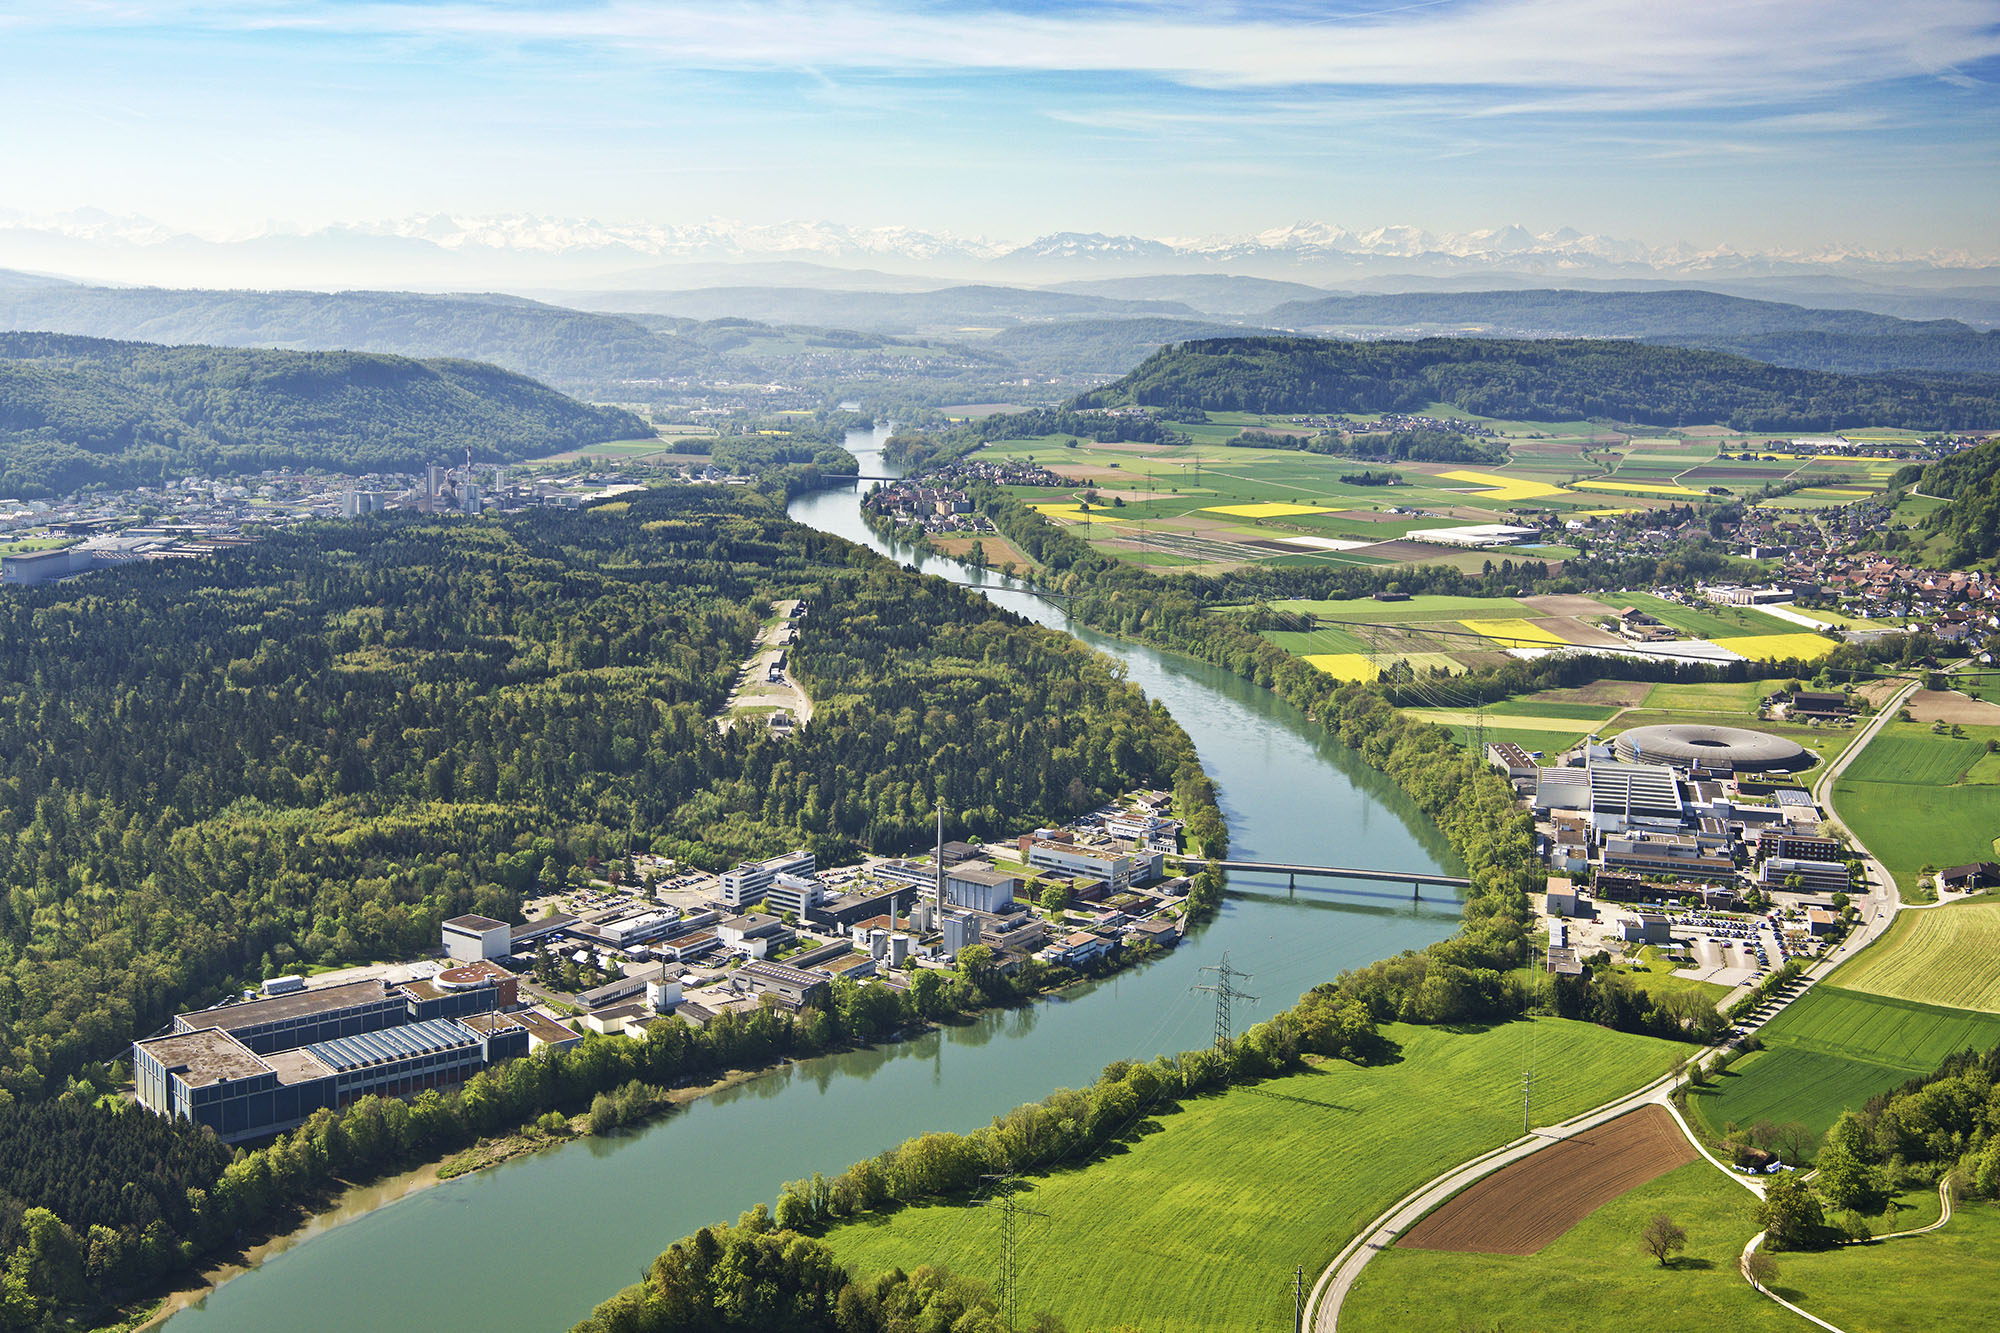
\includegraphics[width=.9\textwidth]{logos/PSI_helicopter}};
          %\node [anchor=south west, inner sep = 4,fill=white, opacity=0.8] at (0.0, 2.0)
                %{
                  %\parbox{3.8cm}{\centering\color{black}
                    %Thank you for your attention.\\
                    
                    %\vspace{1cm}
                           %{\large Questions?}
                           %\vspace{1cm}
                  %}
                  
                %};
  %\end{tikzpicture}
  %\end{adjustbox}
%\end{frame}

%\begin{frame}
  %\frametitle{References}
             %{\scriptsize
               %\begin{multicols}{2}
                 %\bibliography{references.bib}
               %\end{multicols}
             %}
%\end{frame}

%% Here backup slides start.
%\appendix
%\frame{\Large Extra Slides}
%\begin{frame}
  %\frametitlepsi{Results}
    %\Large
    %Backup slides blabla. These slides don't appear on page numbering.

    
    %\includegraphics[width=0.4\textwidth]{plots/posterPlot-SUQ-output.png}
%\end{frame}

%\begin{frame}
  %\frametitlepsi{Results}
    %\Large
    %Backup slides blabla
%\end{frame}

\end{document} 
